% version 1.01 Date 31/03/2016	Auteur Mathieu Medici

Le référentiel Qualité contient l'ensemble des documents produits par l'équipe \nomEquipe{} dans la cadre de sa démarche qualité.

\begin{figure}[ht]
         \begin{center}
         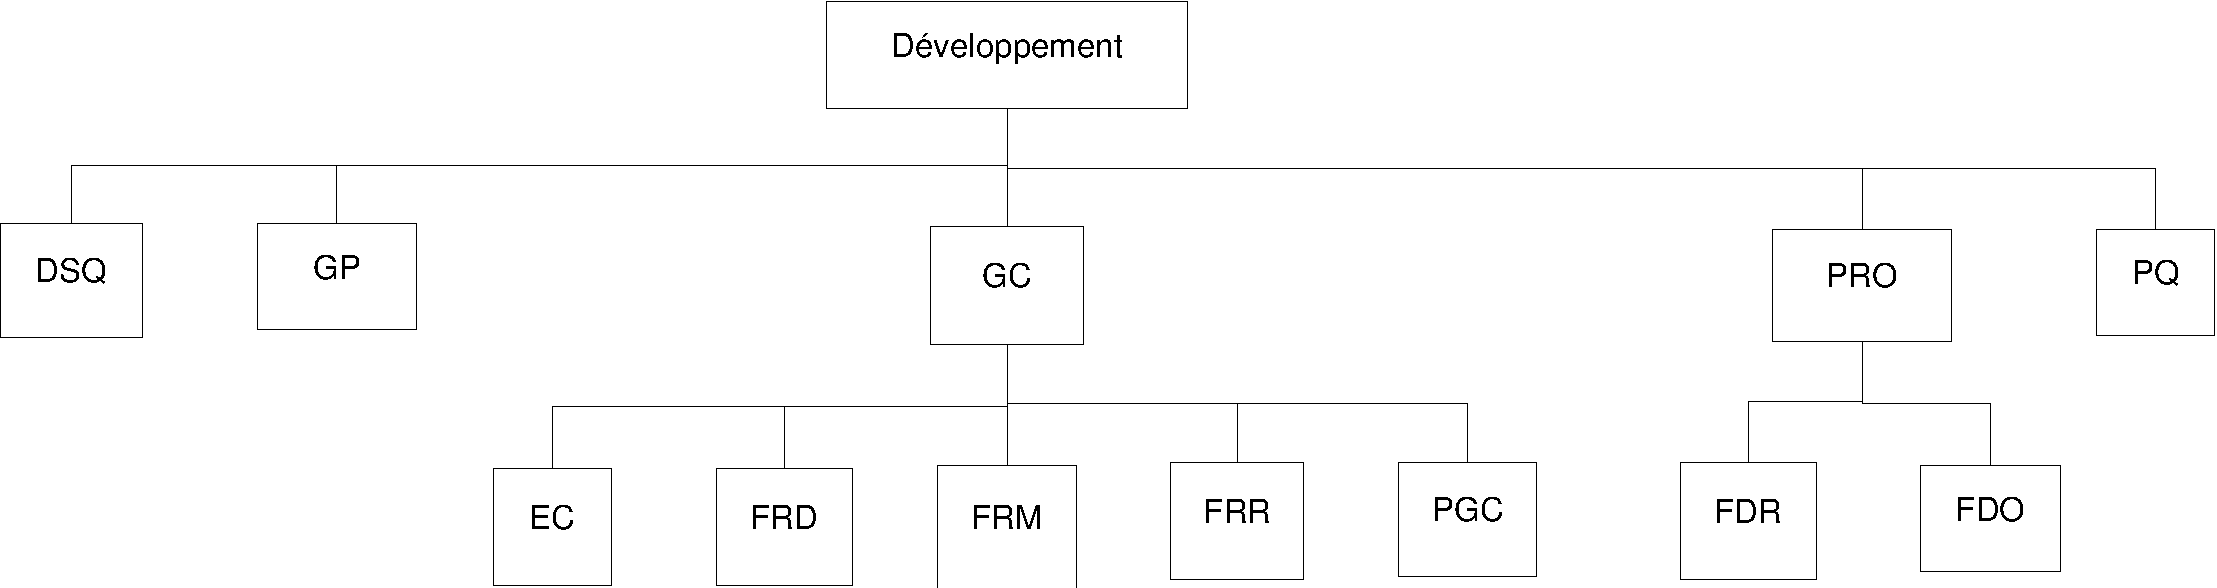
\includegraphics[scale=0.5]{images/arboQualite}
         \end{center}
         \caption{Référentiel Qualité}
 \end{figure}

\clearpage 

\subsection{Structure du répertoire GP}
\addcontentsline{toc}{subsection}{Structure du répertoire GP}

\begin{figure}[ht]
         \begin{center}
         \includegraphics[scale=0.24]{images/arboGP}
         \end{center}
         \caption{Référentiel Qualité - Gestion de Projet}
 \end{figure}
 Le dossier ME contient un dossier pour chaque type de compte-rendu (CRFT, CRC, CRE, CRI, CRIP, CRTP, CRTQ). Ces différents dossiers contiennent chacun : 
 \begin{itemize}
   \item un dossier \emph{mails\_verification} qui contient tous les mails de vérification concernant le type de CR selectionné;
   \item un dossier \emph{mails\_validation} qui contient tous les mails de validation concernant le type de CR selectionné;
   \item un dossier \emph{mails\_approbation} qui contient tous les mails d'approbation concernant le type de CR selectionné.
 \end{itemize}
 
 \subsection{Structure du répertoire DSQ}
\addcontentsline{toc}{subsection}{Structure du répertoire DSQ}

\begin{figure}[ht]
         \begin{center}
         \includegraphics[scale=0.5]{images/arboDSQ}
         \end{center}
         \caption{Référentiel Qualité - Dossier de Suivi de la Qualité}
 \end{figure}

